
%%%%%
%%%%% DO NOT EDIT THIS FILE
%%%%%



\documentclass[12pt,a4paper,fleqn]{report}

%%% packages for mathematical typesetting
\usepackage{amsmath}
\usepackage{amssymb}
\usepackage{times}
\usepackage{bm}
%\usepackage{mathtools}
%\usepackage{nicefrac}
%\usepackage{latexsym}

%%% packages for including figures and subfigures
\usepackage{graphicx}
\usepackage[font=footnotesize,labelformat=empty]{subfig}

%%% package for nicer table layout
\usepackage{booktabs}

%%% package for color mangement
\usepackage[svgnames]{xcolor}

%%% package for page headings and footers
\usepackage{fancyhdr}

%%% package for hyperlinks
\usepackage{hyperref}
\hypersetup{%
  colorlinks=true,
  urlcolor=DarkGreen,
  citecolor=green,
  bookmarks=false}


\usepackage[noend]{algpseudocode}
\algrenewcommand\algorithmicdo{}
\algrenewcommand\algorithmicthen{}
\algrenewcommand{\algorithmiccomment}[1]{// #1}
\makeatletter
\newcommand{\StatexIndent}[1][3]{%
  \setlength\@tempdima{\algorithmicindent}%
  \Statex\hskip\dimexpr#1\@tempdima\relax}
\makeatother


\usepackage{fancyvrb} 
\usepackage{listings}
% Python style / environment for highlighting in "figures"
\lstdefinestyle{pythonstyle}{%
  language=Python,
  tabsize=4,
  backgroundcolor=\color{Gray!10},
  basicstyle=\ttfamily\scriptsize,
  stringstyle=\color{ForestGreen},
  keywordstyle=\color{BlueViolet},
  commentstyle=\itshape\color{DarkRed!90},
  identifierstyle=,
  emphstyle=\color{Blue},
  frame=lines,	
  showstringspaces=false,
  morekeywords={range, len, self, lambda, from, import, as, False, True, enumerate, map, list, set, float, int, min, max, with}
  fancyvrb=true,
}
\lstnewenvironment{python}[1][]{\lstset{style=pythonstyle,#1}}{}





\graphicspath{{./Figures/}, {./Images/}}



%%% text highlighting
\newcommand{\keyword}[1]{\emph{\texttt{\color{blue}#1}}}
\newcommand{\alert}[1]{\emph{\texttt{\color{red}#1}}}


%%% sets
\newcommand{\set}[1]{#1}

%%% vectors, matrices, and tensors
\renewcommand{\vec}[1]{\bm{#1}}
\newcommand{\mat}[1]{\bm{#1}}
\newcommand{\ten}[1]{\bm{\mathcal{#1}}}

%%% trace, rank, and diagonal
\newcommand{\tr}[1]{\operatorname{tr} \bigl [ #1 \bigr ]}
\newcommand{\TR}[1]{\operatorname{tr} \Bigl [ #1 \Bigr ]}
\newcommand{\rk}[1]{\operatorname{rk} \bigl [ #1 \bigr ]}
\newcommand{\RK}[1]{\operatorname{rk} \Bigl [ #1 \Bigr ]}
\newcommand{\diag}[1]{\operatorname{diag} \bigl [ #1 \bigr ]}
\newcommand{\DIAG}[1]{\operatorname{diag} \Bigl [ #1 \Bigr ]}

%%% inverse and transpose
\newcommand{\inv}[1]{#1^{-1}}
\newcommand{\trn}[1]{#1^\intercal}
\newcommand{\invtrn}[1]{#1^{-\intercal}}

%%% outer product
\newcommand{\opt}[2]{#1 \trn{#2}}

%%% inner products
\newcommand{\ipt}[2]{\trn{#1} #2}
\newcommand{\iptb}[2]{\left( \ipt{#1}{#2} \right)}
\newcommand{\ip}[2]{\langle #1, #2 \rangle}
\newcommand{\Ip}[2]{\bigl \langle #1, #2 \bigr \rangle}
\newcommand{\ipa}[2]{\langle #1, #2 \rangle}
\newcommand{\Ipa}[2]{\bigl \langle #1, #2 \bigr \rangle}
\newcommand{\dsq}[2]{\bigl \lVert #1 - #2 \bigr \rVert^2}
\newcommand{\nrm}[1]{\bigl \lVert #1 \bigr \rVert^2}
\newcommand{\sdsq}[2]{\lVert #1 - #2 \rVert^2}
\newcommand{\snrm}[1]{\lVert #1 \rVert^2}


\newcommand{\st}{\operatorname{s.\!t.}}
\newcommand{\amin}[1]{\operatorname*{argmin}_{#1}}
\newcommand{\amax}[1]{\operatorname*{argmax}_{#1}}

\newcommand{\submax}[1]{#1_{\text{max}}}

\newcommand{\ci}{\perp\!\!\!\perp}
\newcommand{\prob}[1]{p\bigl( #1 \bigr)}
\newcommand{\cprob}[2]{p\bigl( #1 \bigm| #2 \bigr)}

%%% horizontal and vertical dash
\newcommand{\hdash}{\operatorname{\,{}---{}\,}}
\renewcommand{\vdash}{\arrowvert}





\pagestyle{fancy}
\lhead{\emph{Pattern Recognition (2)}}
\rhead{\emph{Summer Term 2021}}
\cfoot{}

\frenchspacing

\setlength{\parskip}{1ex plus0.5ex minus0.5ex}

\setlength{\headheight}{15pt}

\def\thesection{\arabic{section}.}
\setlength{\parindent}{0pt}

\renewcommand{\familydefault}{\sfdefault}





\begin{document}

\subsection*{exercise 1}
\textbf{eigenvalues, eigenvectors, and prototypes}
\vspace{1cm}

\subsection*{solutions due}
until \textbf{April 25, 2021} at \textbf{23:59} via \textbf{ecampus}
\vspace{1cm}

\vfill


\subsection*{students handing in this solution set}

\begin{tabular*}{\textwidth}{l@{\extracolsep{\fill}}lll}
  \toprule
  last name & first name & student ID & enrolled with \\
  \midrule
  \midrule
  Nikolskyy
  & Oleksander
  & TODO
  & TODO
  \\
  Schier
  & Marie
  & TODO
  & TODO
  \\
  Doll
  & Niclas
  & 3075509
  & Uni Bonn
  \\
  Safavi
  & Arash
  & TODO
  & TODO
  \\
  Wani
  & Mohamad Saalim
  & TODO
  & TODO
  \\
  Bonani
  & Mayara Everlim
  & TODO
  & TODO
  \\
  \bottomrule
\end{tabular*}
\newpage

%%%%%
%%%%% DO NOT EDIT THE FOLLOWING
%%%%%

\subsection*{general remarks}

As you know, your instructor is an avid  proponent of open science and education. Therefore, \textbf{MATLAB implementations will not be accepted} in this course.

The goal of this exercise is to get used to scientific Python. There are numerous resources on the web related to Python programming. Numpy and Scipy are well documented and Matplotlib, too, comes with numerous tutorials. Play with the code that is provided. Most of the above tasks are trivial to solve, just look around for ideas as to how it can be done.

Remember that you have to achieve at least 50\% of the points of the exercises to be eligible to the written exam at the end of the semester. Your grades (and credits) for this course will be decided based on the exam only, but --once again-- you have to succeed in the exercises to get there.
  
Your solutions have to be \emph{satisfactory} to count as a success. Your code and results will be checked and need to be convincing.

If your solutions meets the above requirements and you can demonstrate that they work in practice, it is a \emph{satisfactory} solution.

A \emph{very good} solution (one that is rewarded full points) requires additional efforts especially w.r.t. to readability of your code. If your code is neither commented nor well structured, your solution is not good! The same holds for your discussion of your results: these should be concise and convincing and demonstrate that you understood what the respective task  was all about. Striving for very good solutions should always be your goal!
 



\subsection*{practical advice}



The problem specifications you'll find below assume that you use python / numpy / scipy for your implementations. They also assume that you have imported the following
\begin{python}
import numpy as np
import numpy.linalg as la
import matplotlib.pyplot as plt
\end{python}


\subsection*{task 1.1 [10 points] \\[1ex] computing spectral- and singular value decompositions}

In the \texttt{Data} folder for this exercise, you will find the file
\begin{quote}
    \texttt{faceMatrix.npy}
\end{quote}
which contains a data matrix $\mat{X} \in \mathbb{R}^{361 \times 2429}$ whose columns $\vec{x}_i$ represent tiny face images of size $19 \times 19$ pixels. To read this matrix into memory and check its size, you may use
\begin{python}
matX = np.load('faceMatrix.npy').astype('float')
m, n = matX.shape
print (m, n)
\end{python}
To have a look at one of the images it contains, say $\vec{x}_{15}$, you may use this
\begin{python}
vecX = matX[:,14].reshape(19,19)
plt.imshow(vecX, cmap='gray')
plt.xticks([])
plt.yticks([])
plt.show()
\end{python}
\vspace{2cm}





Having read matrix $\mat{X}$ into memory, here is what you are supposed to do
\begin{enumerate}
\item normalize $\mat{X}$ such that its column mean is $\vec{0}$
%%%%%
%%%%%
%%%%% enter your code into the following environment
%%%%%
%%%%%
\begin{python}
# normalize the data matrix such that the column mean is zero
# by simply subtracting the mean of each column
X -= X.mean(axis=0, keepdims=True)
\end{python}
%%%%%
%%%%%
%%%%%
%%%%%
%%%%%
\item compute $\mat{C} = \mat{X} \trn{\mat{X}}$ \\ \textbf{NOTE:} we deliberately omit the scaling factor of $\frac{1}{n}$
\item compute the spectral decomposition $\mat{C} = \mat{U} \mat{\Lambda} \,\trn{\mat{U}}$ using \keyword{la.eig}
\item compute the spectral decomposition $\mat{C} = \mat{U} \mat{\Lambda} \,\trn{\mat{U}}$ using \keyword{la.eigh}
\item compare the eigenvalues you obtain from these two approaches; what do you observe ?
\color{blue} \\[1ex]
%%%%%
%%%%%
%%%%% enter your discussion here
%%%%%
%%%%%
Up to permutation the two spectra are exaclty the same (see figure \ref{fig:eig_vs_eigh}). The reason for the different permutations is simply that \keyword{la.eigh} guarantees that the eigenvalues are sorted whereas \keyword{la.eig} doesn't. Also it might happen that some of the elements have flipped signs but we didn't observe this here.

\begin{figure}
    \centering
    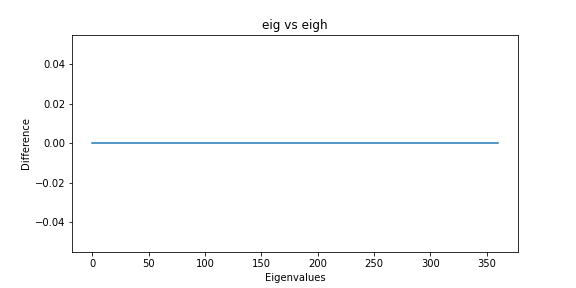
\includegraphics[width=\textwidth]{Ex_01/Figures/eig-vs-eigh.png}
    \caption{Difference of the sorted eigenvalues computed by the two methods. The x-axis lists all the eigenvalues of the matrix $C$ and the y-axis shows the difference of the corresponding values. Really not much to see here.}
    \label{fig:eig_vs_eigh}
\end{figure}
%%%%%
%%%%%
%%%%%
%%%%%
%%%%%
\color{black}
\item compute the singular value decomposition $\mat{X} = \mat{U} \mat{\Sigma} \trn{\mat{V}}$ using \keyword{la.svd}
\item square the resulting singular values and compare them to the eigenvalues you found above; what do you observe ?
\color{blue} \\[1ex]
%%%%%
%%%%%
%%%%% enter your discussion here
%%%%%
%%%%%
As the theory suggests we observe that the squared singular values equal the eigenvalues of the matrix $C$ (again up to permutation). Nevertheless we see distortions between the two sets (see figure \ref{fig:eigh_vs_svd}). This is probably due to numerical error, since \keyword{la.svd} doesn't directly compute the eigenvalues but their square root. The magnitude of the eigenvalues that show differences also support our hypothesis. Still the differences are negligible.

\begin{figure}
    \centering
    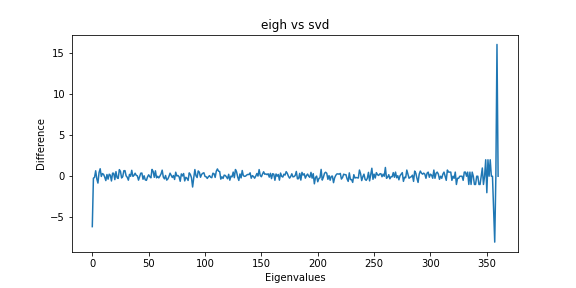
\includegraphics[width=\textwidth]{Ex_01/Figures/eigh-vs-svd.png}
    \caption{Difference between the eigenvalues computed by \keyword{la.eigh} and \keyword{la.svd}. Other than before there actually are differences between the two spectra. But w.r.t to the magnitude of the values, the error is negligible. Note that the eigenvalues are sorted in ascending order.}
    \label{fig:eigh-vs-svd}
\end{figure}
%%%%%
%%%%%
%%%%%
%%%%%
%%%%%
\color{black}
\item create a plot of the three spectra you just computed; do you get any warnings or error messages ?
%%%%%
%%%%%
%%%%% enter plot here, i.e. replace "placeholder.pdf" by the name of the graphics file you created
%%%%%
%%%%%
\begin{center}
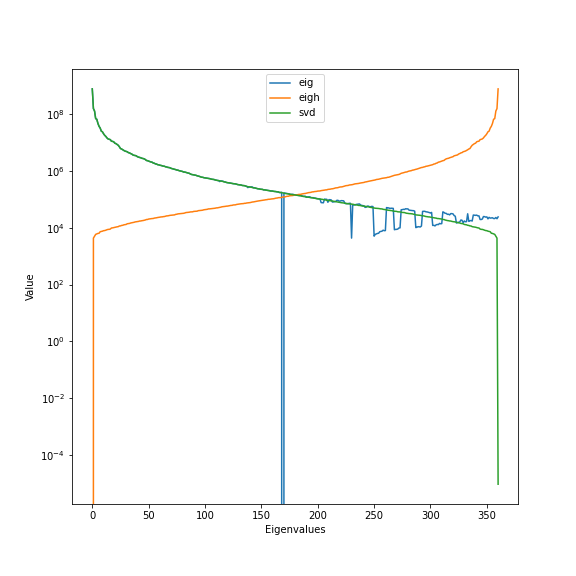
\includegraphics[width=0.75\textwidth]{Ex_01/Figures/eig.png}
\end{center}
%%%%%
%%%%%
%%%%%
%%%%%
%%%%%
\end{enumerate}



\subsection*{task 1.2 [10 points] \\[1ex] timing spectral- and singular value decompositions}

Proceed just as above, but now measure the (average) run-time of the methods \keyword{la.eig}, \keyword{la.eigh}, and \keyword{la.svd}.

Here, it is highly recommended you make use of Python's \keyword{timeit} module. Examples for its proper use can be found in 
\begin{itemize}
\item[] C. Bauckhage, \href{https://www.researchgate.net/publication/329449786_NumPy_SciPy_Recipes_for_Image_Processing_Avoiding_for_Loops_over_Pixel_Coordinates}{\textbf{``NumPy / SciPy Recipes for Image Processing: Avoiding for Loops over Pixel Coordinates''}}, technical report, 2018 
\end{itemize}

Make sure that your run-time comparisons are fair! In other words, pay attention to the fact that \keyword{la.eig} and \keyword{la.eigh} require to compute matrix $\mat{C}$ from $\mat{X}$ whereas \keyword{la.svd} works directly on $\mat{X}$.
%%%%%
%%%%%
%%%%% enter your code into the following environment
%%%%%
%%%%%
\begin{python}
from timeit import timeit
n = 100
eig_time = timeit(lambda: la.eig(X @ X.T), number=n)
eigh_time = timeit(lambda: la.eigh(X @ X.T), number=n)
svd_time = timeit(lambda: la.svd(X)[1] ** 2, number=n)
# print the average time spend for each method
print("la.eig:  %.3fs" % eig_time / n)
print("la.eigh: %.3fs" % eigh_time / n)
print("la.svd:  %.3fs" % svd_time / n)
\end{python}
%%%%%
%%%%%
%%%%%
%%%%%
%%%%%
\vspace{2cm}
Run your code. What do you observe ? Do your result so far suggest any preference for any of the methods considered up to this point ?
\color{blue} \\[1ex]
%%%%%
%%%%%
%%%%% enter your discussion here
%%%%%
%%%%%
The code outputs the following:

la.eig:  0.090s \\
la.eigh: 0.024s \\
la.svd:  0.909s \\

We see that singular value decomposition is by far the slowest method. This observation can be explained by the dimensions of the matrix $X$ ($361 \times 2429$) in comparison to $C$ ($361 \times 361$). 

The fastest method is \keyword{la.eigh}. Reason for this is that \keyword{la.eigh} assumes the input matrix to be symmetric/hermitian and thus can use a faster algorithm than \keyword{la.eig}. On the other hand \keyword{la.eig} doesn't assume anything on the input matrix other than it being square.

Together with the observations from exercise 1, the prefered method for this specific problem instance is \keyword{la.eigh} for the already mentioned reasons.
%%%%%
%%%%%
%%%%%
%%%%%
%%%%%
\color{black}
\newpage




\subsection*{task 1.3 [10 points] \\[1ex] implementing the QR algorithm}

Given the matrix $\mat{C}$ as computed in task 1.1, implement the following iterative procedure

\vspace{1ex}

\hrule
\begin{algorithmic}
\State $\mat{C}_0 = \mat{C}$
\State
\For{$t = 1, \ldots, 10$}
\State
\State compute the QR decomposition of $\mat{C}_{t-1}$ to obtain matrices $\mat{Q}_t$ and $\mat{R}_t$
\State
\State given matrices $\mat{Q}_t$ and $\mat{R}_t$, compute
\begin{equation*}
\mat{C}_t = \mat{R}_t \mat{Q}_t
\end{equation*} 
\EndFor
\end{algorithmic}
\hrule
\vspace{1ex}
%%%%%
%%%%%
%%%%% enter your code into the following environment
%%%%%
%%%%%
\begin{python}
# past your code here


\end{python}
%%%%%
%%%%%
%%%%%
%%%%%
%%%%%
\vfill

Run your code and have a look at the diagonal entries of the resulting matrix $\mat{C}_{10}$. Compare them against the spectra you computed above; what do you observe ?
\color{blue} \\[1ex]
%%%%%
%%%%%
%%%%% enter your discussion here
%%%%%
%%%%%
enter your discussion here \ldots
%%%%%
%%%%%
%%%%%
%%%%%
%%%%%
\color{black}
\vspace{2cm}

Now, consider the following equivalencies
\begin{equation*}
\mat{C}_t = \mat{R}_t \mat{Q}_t = \inv{\mat{Q}_t} \mat{Q}_t \mat{R}_t \mat{Q}_t = \mat{Q}_t^{-1} \mat{C}_{t-1} \mat{Q}_t = \trn{\mat{Q}_t} \mat{C}_{t-1} \mat{Q}_t 
\end{equation*}
Can you use this insight to explain the result you get form running the QR algorithm ?
\color{blue} \\[1ex]
%%%%%
%%%%%
%%%%% enter your discussion here
%%%%%
%%%%%
enter your discussion here \ldots
%%%%%
%%%%%
%%%%%
%%%%%
%%%%%
\color{black}
\newpage



\subsection*{bonus [5 points]}

If you want to impress your instructors, perform run-time measurements for your implementation of the QR algorithm as well.
\color{blue} \\[1ex]
%%%%%
%%%%%
%%%%% enter your discussion here
%%%%%
%%%%%
enter your discussion here \ldots
%%%%%
%%%%%
%%%%%
%%%%%
%%%%%
\color{black}





\subsection*{task 1.4 [20 points] \\[1ex] finding maximally different images}

So far, you only had to do what the problem specifications asked you to do. In this task, you need to get creative!

Reread matrix $\mat{X}$ from task 1.1 into memory but \emph{do not normalize it to zero mean}. Now, think of / invent an algorithm that selects $k>2$ out of the $n$ columns of $\mat{X}$ such that the selected data vectors are as far apart as possible. 

Mathematically, the problem considered in this task is a subset selection problem and we can formalize it as follows: given $X = \{ \vec{x}_1, \ldots, \vec{x}_n \}$, solve
\begin{align*}
S^* = \amax{S \subset X} & \sum_{\vec{x}_i \in S} \sum_{\vec{x}_j \in S} \dsq{\vec{x}_i}{\vec{x}_j} \\
\st \; & \; \; \lvert S \rvert = k
\end{align*}
\textbf{NOTE:} this problem is actually way more difficult than it may appear at first sight; in fact, it is NP-complete and an \textit{efficient} algorithm that is \textit{guaranteed} to find the optimal $S^*$ for very large sets $X$ and arbitrary choices of $k$ remains elusive to this date. \vspace{1ex}

%%%%%
%%%%%
%%%%% enter your code into the following environment
%%%%%
%%%%%
\begin{python}
# past your code here


\end{python}
%%%%%
%%%%%
%%%%%
%%%%%
%%%%%
\vspace{2cm}

Test your algorithm for several choices of $k$, say $k \in \{ 25, 50, 100 \}$, and visualize the extracted columns in terms of tiny images. For instance, for $k \in \{ 4, 9, 16 \}$, your result could look like this:
%%%%%
%%%%%
%%%%% enter your plots here, i.e. replace "t1-4-k*.png" by the names of the graphics files you created
%%%%%
%%%%%

%%%%%
%%%%%
%%%%%
%%%%%
%%%%%
Simply replace the above three images with your results for $k \in \{25, 50, 100\}$.








\end{document}
